\section{Overview of Real-Time Operating Systems}
% \section*{Overview of Real-Time Operating Systems}
% \addcontentsline{toc}{section}{Overview of Real-Time Operating Systems}
% Remove header text
\markboth{}{}
    Real-time systems are systems with rigid timing requirements
        \cite[pp. 46]{textbook}.
    RTOSs can be used to provide a layer of abstraction between the software
        handling real-time events and the underlying hardware.
    These operating systems must be high-performance with predictable and
        deterministic behavior \cite{rtos-definition}.

    Real-time systems can be categorized into \textit{soft} and \textit{hard}
        systems.
    According to Intel, hard real-time systems refer to systems where missing a
        deadline means failure of the system \cite{intel-hard-soft-real-time}.
    In soft real-time systems, however, the focus in on optimizing quality of
        service.
    Missing a deadline would result lower-quality service, not in a system
        failure \cite{hard-soft-real-time}.
    As an example, a robotic arm needs to be instructed to stop \textit{before}
        it hits a wall, and failure to meet this deadline will cause the arm to
        break.
    This means the robotic arm is a hard real-time system
        \cite[pp. 45-46]{textbook}.
    A consumer smartphone would be a soft real-time system because while a
        lagging phone is frustrating to the user, it is not catastrophic.

    There are many strategies for implementing a RTOS.
    The focus is on responding to external (real-time) events in a time period
        that is minimal and predictable.
    The time taken to respond to an event is called \textit{dispatch latency}.
    As shown in \fig{rtos_dispatch_latency}, dispatch latency consists of many
        aspects, like interrupt processing, preempting and managing conflicts
        with other processes, and executing the actual process.
    Thus, the operating system's process scheduling algorithm is of utmost
        importance.

    \begin{figure}[H]
        \centering
        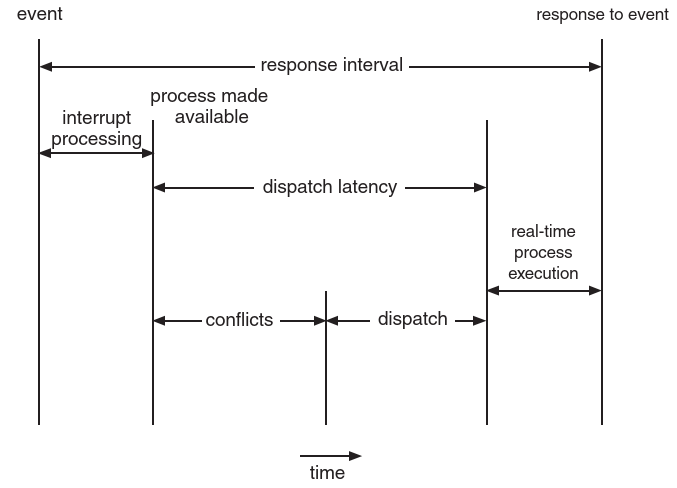
\includegraphics
            [width=0.7\textwidth]
            {images/rtos_dispatch_latency.png}
        \caption
            [Dispatch latency of an event]
            {Dispatch latency of an event \cite[p. 229]{textbook}.}
        \label{fig:rtos_dispatch_latency}
    \end{figure}

    To meet strict deadline requirements, a priority-based scheduler is
        necessary.
    Such a scheduler enables higher-priority processes to preempt lower-priority
        ones \cite[p. 229]{textbook}.
    For hard real-time systems, both the CPU burst time of the process and its
        deadline must be known.
    When a process is ready to execute, the scheduler can decide whether or not
        it is possible to meet the process's deadline, and choose to schedule it
        accordingly.
    This is called an \textit{admission-control algorithm}
        \cite[pp. 229-230]{textbook}.

    \textit{Rate-monotonic} scheduling can be used to schedule periodic real-time tasks.
    In this algorithm, processes with shorter periods are assigned higher
        priorities, since they have a shorter deadline.
    For this type of scheduling to work its CPU burst time must be the same
        every time it executes, and must be shorter than its deadline and
        period.
    A pitfall of rate-monotonic scheduling is that it is not always able
        schedule processes even if there is enough CPU time for them
        \cite[pp. 230-232]{textbook}.

    Another real-time scheduling technique is called
        \textit{earliest-deadline-first (EDF)}.
    In this algorithm, higher priority is given to processes whose deadline is
        sooner.
    This way, a process near its deadline can preempt a process that has more
        time to spare.
    EDF scheduling can achieve a CPU usage near 100\%, thus being able to
        schedule more processes than rate-monotonic scheduling
        \cite[pp. 232-233]{textbook}.

    Implementing an RTOSs is more complex than using a Linux-based operating
        system, but the complexity is the cost for performance.
    For hard real-time systems, an RTOS is necessary to meet performance
        requirements.
    For soft real-time systems, tradeoffs must be balanced to determine whether
        the improved service quality of the system is worth the added complexity
        and cost.
